% =====================================================================
% PEIB (SEES0082) Lecture 7 - Prices vs quantities (Weitzman 1974), English
% Translated on 24 Nov 2026 from the French Namur audition deck (26 Jan 2026),
% source: Latex slides/Environmental Economics/main.tex, section "Namur Audition".
% Diagrams keep that deck's colours: blue = cost curves, red = damage,
% green = policy line / tax loss, yellow = quota loss, gray dashed = guides.
%
% Part A (core, shown in the lecture): labels w7_mac_md, w7_md_steep,
%   w7_md_flat, w7_table
% Part B (additional frames, same order as the Namur talk): w7_agenda,
%   w7_why, w7_externality, w7_price_or_quantity, w7_uncertainty,
%   w7_compare, w7_conclusion
%
% Build (skill latex-teaching):
%   py "$HOME/.claude/skills/latex-teaching/scripts/build.py" lecture07_weitzman.tex
%   py "$HOME/.claude/skills/latex-teaching/scripts/build.py" lecture07_weitzman.tex --handout
% Export the four core frames for PowerPoint (handout PDF = one page per frame):
%   py "$HOME/.claude/skills/latex-teaching/scripts/export_frames.py" lecture07_weitzman_handout.pdf
%      --out ../png/week7 --pages 1-4 --names w7_mac_md,w7_md_steep,w7_md_flat,w7_table
% =====================================================================
\documentclass{beamer}

\usepackage{tikz}
\usepackage{pgfplots}
\usepackage{amsmath}
\usepackage{amssymb}
\usepackage{xcolor}
\usepackage{booktabs}
\usepackage{colortbl}
\usepackage{array}

\usetikzlibrary{decorations.pathreplacing}
\pgfplotsset{compat=newest}

% Minimal, no headers/footers/nav symbols
\mode<presentation>{
  \usetheme{default}
  \setbeamertemplate{navigation symbols}{}
  \setbeamertemplate{headline}{}
  \setbeamertemplate{footline}{}
}

% Core frames only: uncomment
% \includeonlyframes{w7_mac_md,w7_md_steep,w7_md_flat,w7_table}

\begin{document}

% =====================================================================
% PART A: core frames
% =====================================================================

%========================
% A1: MAC and MD against pollution reduction, optimum and market level
% R* = (k - bA)/(2m) = (3.8 - 0.8)/1 = 3.0 ; P* = 0.5*3 + 0.8 = 2.3
% Rm = R* - 1.2 = 1.8 ; Pm = 0.5*1.8 + 0.8 = 1.7
%========================
\begin{frame}[label=w7_mac_md]{How do we reach the socially optimal level of pollution?}
\centering
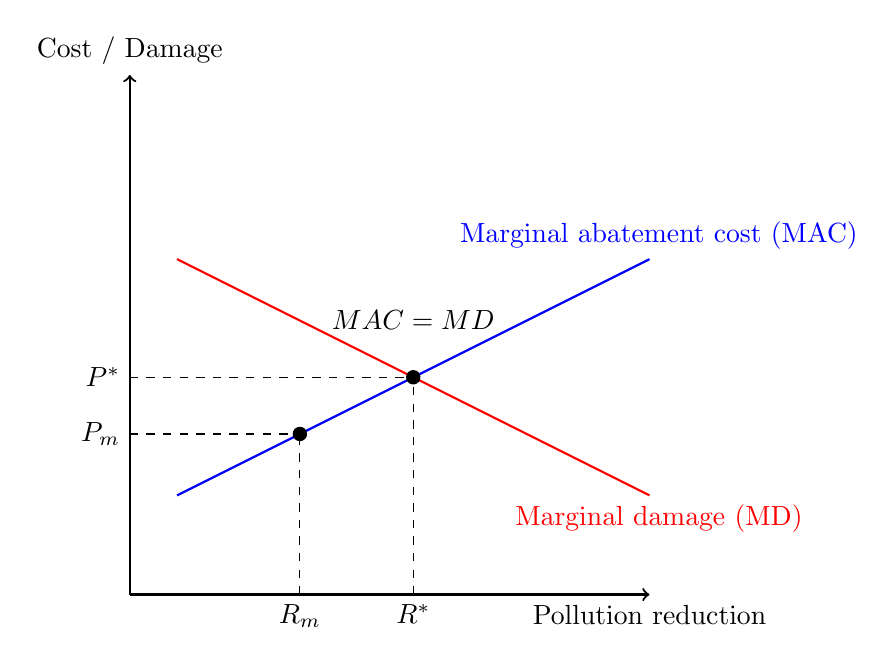
\begin{tikzpicture}[scale=1.2]

% Parameters
\pgfmathsetmacro{\m}{0.5}   % slope
\pgfmathsetmacro{\bA}{0.8}  % intercept MAC
\pgfmathsetmacro{\k}{3.8}   % intercept MD

% Intersection MAC = MD (social optimum)
\pgfmathsetmacro{\Rstar}{(\k-\bA)/(2*\m)}
\pgfmathsetmacro{\Pstar}{\m*\Rstar+\bA}

% Market level (Rm < R*)
\pgfmathsetmacro{\Rm}{\Rstar-1.2}
\pgfmathsetmacro{\Pm}{\m*\Rm+\bA}

% Axes (always visible)
\draw[->, thick] (0,0) -- (5.5,0) node[below] {Pollution reduction};
\draw[->, thick] (0,0) -- (0,5.5) node[above] {Cost / Damage};

% 1) MAC
\onslide<2->{
\draw[thick, blue] (0.5, {\m*0.5+\bA}) -- (5.5, {\m*5.5+\bA});
\node[blue] at (5.6, {\m*5.5+\bA+0.25}) {Marginal abatement cost (MAC)};
}
% 2) MD
\onslide<3->{
\draw[thick, red] (0.5, {\k-\m*0.5}) -- (5.5, {\k-\m*5.5});
\node[red] at (5.6, {\k-\m*5.5-0.25}) {Marginal damage (MD)};
}

% 3) Social optimum (R*, P*, MAC = MD)
\onslide<4->{
\filldraw[black] (\Rstar,\Pstar) circle (2pt);
\draw[dashed] (\Rstar,0) -- (\Rstar,\Pstar);
\node[below] at (\Rstar,0) {$R^*$};
\draw[dashed] (0,\Pstar) -- (\Rstar,\Pstar);
\node[left] at (0,\Pstar) {$P^*$};
}

% Label MAC = MD above the intersection (step 4 only)
\onslide<4>{
\node[above] at (\Rstar, \Pstar + 0.4) {$MAC = MD$};
}

% 4) Market level (Rm, Pm)
\onslide<5->{
\filldraw[black] (\Rm,\Pm) circle (2pt);
\draw[dashed] (\Rm,0) -- (\Rm,\Pm);
\node[below] at (\Rm,0) {$R_m$};
\draw[dashed] (0,\Pm) -- (\Rm,\Pm);
\node[left] at (0,\Pm) {$P_m$};
}

\end{tikzpicture}
\end{frame}

%========================
% A2: tax vs quota, steep MD  =>  quantities
% tax through pivot: t = 0.6*2.5 + 0.2 = 1.7 ; k = 1.7 + 1.2*2.5 = 4.7
% Ro = (4.7-1.2)/1.8 = 1.94 ; Rt = (1.7-1.2)/0.6 = 0.83 ; Rq = 2.5
%========================
\begin{frame}[label=w7_md_steep]{Tax vs quota: steep MD curve}
\centering
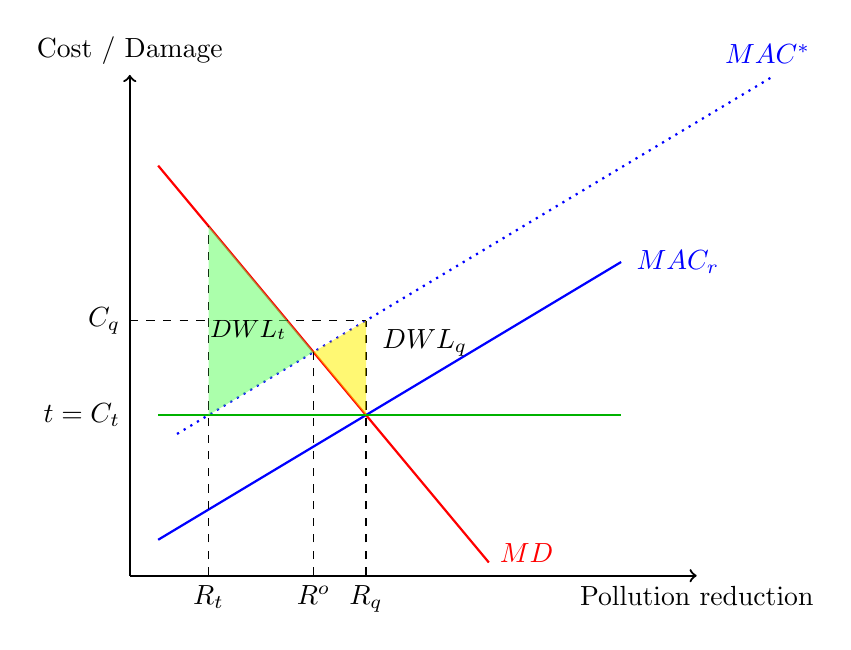
\begin{tikzpicture}[scale=1.2]
% Parameters
\pgfmathsetmacro{\m}{0.6}        % slope of the MAC curves
\pgfmathsetmacro{\bE}{0.2}       % intercept MAC_r (regulator's estimate)
\pgfmathsetmacro{\bA}{1.2}       % intercept MAC* (true cost)

% Pivot: intersection of MAC_r and the tax
\pgfmathsetmacro{\Rpivot}{2.5}
\pgfmathsetmacro{\tlevel}{\m*\Rpivot+\bE}

% Slope of MD (steep)
\pgfmathsetmacro{\d}{1.2}
% k so that MD passes through the pivot (Rpivot, tlevel)
\pgfmathsetmacro{\k}{\tlevel + \d*\Rpivot}

% R^o (optimum): MAC* = MD
\pgfmathsetmacro{\Ro}{(\k-\bA)/(\m+\d)}
\pgfmathsetmacro{\yRo}{\m*\Ro+\bA}
% R_t: MAC* = tax (left of R^o)
\pgfmathsetmacro{\Rt}{(\tlevel-\bA)/\m}
\pgfmathsetmacro{\yMDatRt}{\k-\d*\Rt}
% R_q: MAC_r = MD (right of R^o)
\pgfmathsetmacro{\Rq}{(\k-\bE)/(\m+\d)}
\pgfmathsetmacro{\yRq}{\m*\Rq+\bE}
\pgfmathsetmacro{\Cq}{\m*\Rq+\bA}  % cost on MAC* at R_q

% Axes
\draw[->, thick] (0,0) -- (6,0) node[below] {Pollution reduction};
\draw[->, thick] (0,0) -- (0,5.3) node[above] {Cost / Damage};

% MAC* (dotted)
\draw[thick, blue, dotted] (0.5, {\m*0.5+\bA}) -- (6.8, {\m*6.8+\bA});
\node[blue] at (6.75, {\m*7.2+\bA}) {$MAC^*$};
% MAC_r
\draw[thick, blue] (0.3, {\m*0.3+\bE}) -- (5.2, {\m*5.2+\bE});
\node[blue] at (5.8, {\m*5.2+\bE}) {$MAC_r$};
% MD (steep)
\draw[thick, red] (0.3, {\k-\d*0.3}) -- (3.8, {\k-\d*3.8});
\node[red] at (4.2, {\k-\d*3.8+0.1}) {$MD$};
% Tax
\draw[thick, green!70!black] (0.3,\tlevel) -- (5.2,\tlevel);
\node[left] at (0,\tlevel) {$t=C_t$};

% Verticals
\draw[dashed] (\Rt,0) -- (\Rt,\yMDatRt);
\node[below] at (\Rt,0) {$R_t$};
\draw[dashed] (\Ro,0) -- (\Ro,\yRo);
\node[below] at (\Ro,0) {$R^{o}$};
\draw[dashed] (\Rq,0) -- (\Rq,\Cq);
\node[below] at (\Rq,0) {$R_q$};
% Horizontal C_q
\draw[dashed] (0,\Cq) -- (\Rq,\Cq);
\node[left] at (0,\Cq) {$C_q$};

% Welfare loss of the tax
\fill[green!60, opacity=0.55]
  (\Rt,\tlevel) -- (\Ro,\yRo) -- (\Rt,\yMDatRt) -- cycle;
\node at ({\Rt+0.42}, {(\tlevel+\yMDatRt)/2 - 0.1}) {\small $DWL_t$};
% Welfare loss of the quota
\fill[yellow, opacity=0.55]
  (\Ro,\yRo) -- (\Rq,\yRq) -- (\Rq,\Cq) -- cycle;
\node at ({(\Ro+\Rq)/2 + 0.9}, {\yRo+0.1}) {$DWL_q$};

\end{tikzpicture}

\vspace{-0.2cm}
{\footnotesize $MAC_r$: regulator's estimate (sets the tax $t$ or the quota $R_q$); $MAC^*$: true cost. \\
Steep MD: $DWL_t > DWL_q$ $\Rightarrow$ regulate the \textbf{quantity}.}
\end{frame}

%========================
% A3: tax vs quota, flat MD  =>  prices
% Rq = (3.2-0.2)/0.8 = 3.75 ; t = 0.6*3.75 + 0.2 = 2.45
% Ro = (3.2-1.2)/0.8 = 2.5 ; Rt = (2.45-1.2)/0.6 = 2.08
%========================
\begin{frame}[label=w7_md_flat]{Tax vs quota: flat MD curve}
\centering
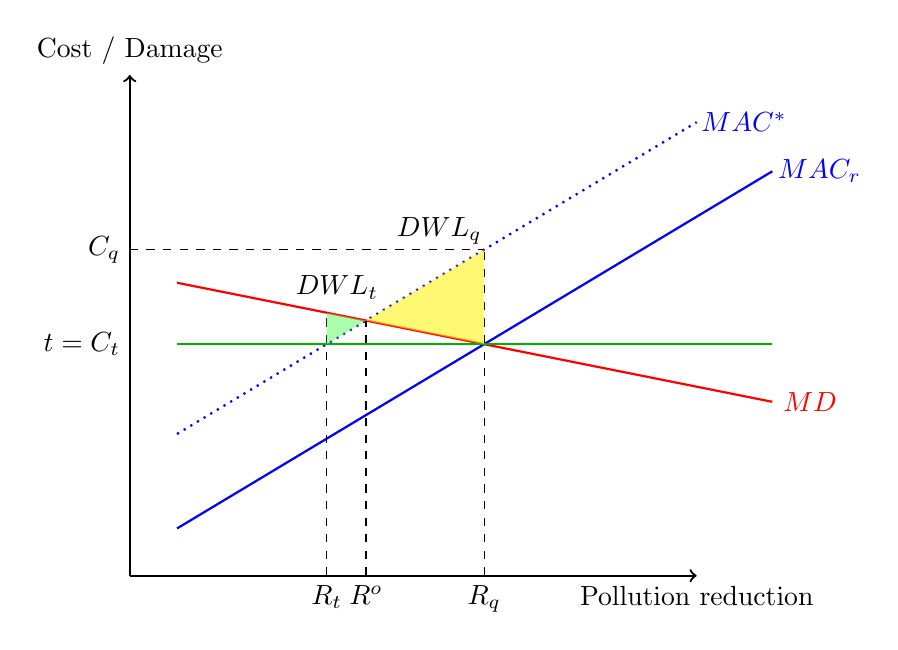
\begin{tikzpicture}[scale=1.2]

% Parameters (MD relatively flat)
\pgfmathsetmacro{\m}{0.6}
\pgfmathsetmacro{\bE}{0.2}
\pgfmathsetmacro{\bA}{1.2}
\pgfmathsetmacro{\k}{3.2}
\pgfmathsetmacro{\d}{0.2}

% Pivot: intersection of MAC_r and MD
\pgfmathsetmacro{\Rpivot}{(\k-\bE)/(\m+\d)}
\pgfmathsetmacro{\tlevel}{\m*\Rpivot+\bE}

\pgfmathsetmacro{\Ro}{(\k-\bA)/(\m+\d)}
\pgfmathsetmacro{\yRo}{\m*\Ro+\bA}
\pgfmathsetmacro{\Rq}{(\k-\bE)/(\m+\d)}
\pgfmathsetmacro{\yRq}{\m*\Rq+\bE}
% R_t: MAC* = tax
\pgfmathsetmacro{\Rt}{(\tlevel-\bA)/\m}
\pgfmathsetmacro{\yMDatRt}{\k-\d*\Rt}
\pgfmathsetmacro{\Cq}{\m*\Rq+\bA}

% Axes
\draw[->, thick] (0,0) -- (6,0) node[below] {Pollution reduction};
\draw[->, thick] (0,0) -- (0,5.3) node[above] {Cost / Damage};

% Curves
\draw[thick, blue, dotted] (0.5, {\m*0.5+\bA}) -- (6.0, {\m*6.0+\bA});
\node[blue] at (6.5, {\m*6.0+\bA}) {$MAC^*$};
\draw[thick, blue] (0.5, {\m*0.5+\bE}) -- (6.8, {\m*6.8+\bE});
\node[blue] at (7.3, {\m*6.8+\bE}) {$MAC_r$};
\draw[thick, red] (0.5, {\k-\d*0.5}) -- (6.8, {\k-\d*6.8});
\node[red] at (7.2, {\k-\d*6.8}) {$MD$};

% Tax
\draw[thick, green!70!black] (0.5,\tlevel) -- (6.8,\tlevel);
\node[left] at (0,\tlevel) {$t=C_t$};

% Verticals
\draw[dashed] (\Rt,0) -- (\Rt,\yMDatRt);
\node[below] at (\Rt,0) {$R_t$};
\draw[dashed] (\Ro,0) -- (\Ro,\yRo);
\node[below] at (\Ro,0) {$R^{o}$};
\draw[dashed] (\Rq,0) -- (\Rq,\Cq);
\node[below] at (\Rq,0) {$R_q$};
% Horizontal C_q
\draw[dashed] (0,\Cq) -- (\Rq,\Cq);
\node[left] at (0,\Cq) {$C_q$};

% Welfare loss of the tax
\fill[green!60, opacity=0.55]
(\Rt,\tlevel) -- (\Ro,\yRo) -- (\Rt,\yMDatRt) -- cycle;
\node at ({(\Rt+\Ro)/2 -0.1}, {\tlevel+0.6}) {$DWL_t$};
% Welfare loss of the quota
\fill[yellow, opacity=0.55]
(\Ro,\yRo) -- (\Rq,\yRq) -- (\Rq,\Cq) -- cycle;
\node at ({(\Ro+\Rq)/2 +0.15}, {\yRo+0.95}) {$DWL_q$};

\end{tikzpicture}

\vspace{-0.2cm}
{\footnotesize $MAC_r$: regulator's estimate (sets the tax $t$ or the quota $R_q$); $MAC^*$: true cost. \\
Flat MD: $DWL_t < DWL_q$ $\Rightarrow$ regulate the \textbf{price}.}
\end{frame}

%========================
% A4: contingency table MAC vs MD
%========================
\begin{frame}[label=w7_table]{Price or quantity? The role of the slopes}

\centering
\renewcommand{\arraystretch}{1.8}
\begin{tabular}{>{\centering\arraybackslash}m{3cm}|>{\centering\arraybackslash}m{3.5cm}|>{\centering\arraybackslash}m{3.5cm}}
\toprule
 & \textbf{Flat MAC} \newline \small{($C''$ small)} & \textbf{Steep MAC} \newline \small{($C''$ large)} \\
\midrule
\textbf{Flat MD} \newline \small{($|B''|$ small)}
& \cellcolor{gray!20} Instruments equivalent
& \cellcolor{green!25} \textbf{Prices preferable} \\
\midrule
\textbf{Steep MD} \newline \small{($|B''|$ large)}
& \cellcolor{yellow!35} \textbf{Quantities preferable}
& \cellcolor{gray!20} Instruments equivalent \\
\bottomrule
\end{tabular}

\vspace{0.5cm}

\begin{itemize}
  \item Steep MD: errors in the level of pollution are very costly $\Rightarrow$ quantities.
  \item Steep MAC: errors in the cost of abatement are very costly $\Rightarrow$ prices.
\end{itemize}

\end{frame}

% =====================================================================
% PART B: additional frames (order of the Namur talk)
% =====================================================================

\begin{frame}[label=w7_agenda]{Regulating pollution under uncertainty: agenda}

\textbf{Topic:} regulating pollution under uncertainty \\ (Martin Weitzman 1974, \textit{Prices vs. Quantities})

\begin{enumerate}
    \item Pollution as an externality that causes a market failure and overproduction \\~\\
    \item Weitzman's question: regulate pollution through prices or through quantities? \\~\\
    \item Key result: the choice of instrument depends on the relation between abatement costs \& the damages from pollution
\end{enumerate}

\end{frame}


\begin{frame}[label=w7_why]{Why care about pollution?}
\begin{itemize}
    \item Since the industrial revolution: unprecedented economic growth and rise in incomes and material well-being \\~\\

    \item Accompanied by equally unprecedented environmental pollution \\~\\

    \item Massive consequences for humans (health) \& nature (climate, biodiversity) \\~\\

    \item The economic view of pollution: an \textbf{externality}
        \begin{itemize}
            \item Definition: an agent's actions affect the well-being of third parties, and the agent does not take this into account in her decisions
            \item As a result, the decisions of market actors lead to excess pollution
        \end{itemize}
\end{itemize}
\end{frame}


%========================
% B: externality and overproduction
% Qm = (4.5-0.3)/1.3 = 3.23 ; Pm = 2.24 ; Q* = (4.5-0.3-1.4)/1.3 = 2.15 ; P* = 2.99
%========================
\begin{frame}[label=w7_externality]{The externality and overproduction (and overpollution)}
\centering
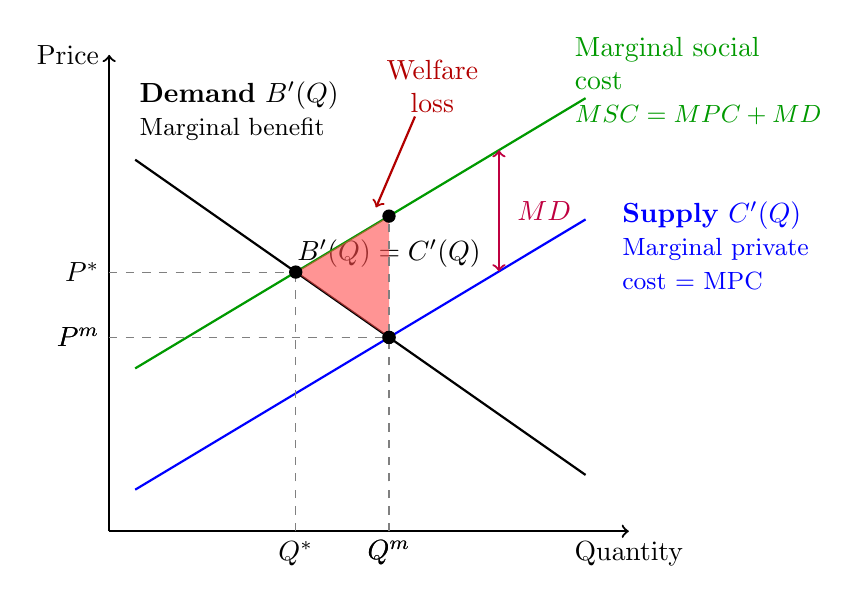
\begin{tikzpicture}[scale=1.1]

% Parameters
\pgfmathsetmacro{\mD}{-0.7}    % slope demand
\pgfmathsetmacro{\bD}{4.5}     % intercept demand
\pgfmathsetmacro{\mS}{0.6}     % slope supply (MPC)
\pgfmathsetmacro{\bS}{0.3}     % intercept supply
\pgfmathsetmacro{\dm}{1.4}     % vertical shift for MSC

% Market: demand = supply (MPC)
\pgfmathsetmacro{\Qm}{(\bD-\bS)/(\mS-\mD)}
\pgfmathsetmacro{\Pm}{\mS*\Qm+\bS}
% Optimum: demand = MSC
\pgfmathsetmacro{\Qstar}{(\bD-\bS-\dm)/(\mS-\mD)}
\pgfmathsetmacro{\Pstar}{\mS*\Qstar+\bS+\dm}
% MSC at Qm (for the triangle)
\pgfmathsetmacro{\MSCatQm}{\mS*\Qm+\bS+\dm}

% Axes
\draw[->, thick] (0,0) -- (6,0) node[below] {Quantity};
\draw[->, thick] (0,0) -- (0,5.5) node[left] {Price};

% Demand B'(Q)
\draw[thick, black] (0.3, {\mD*0.3+\bD}) -- (5.5, {\mD*5.5+\bD});
\node[black, align=left] at (1.5, {\mD*0.5+\bD+0.7}) {\textbf{Demand} $B'(Q)$ \\ \small Marginal benefit};

% Supply MPC = C'(Q)
\draw[thick, blue] (0.3, {\mS*0.3+\bS}) -- (5.5, {\mS*5.5+\bS});
\node[blue, align=left] at (7, {\mS*5.0+\bS}) {\textbf{Supply} $C'(Q)$ \\ \small Marginal private \\ \small cost = MPC};

% Market equilibrium (step 1 only)
\onslide<1>{
\draw[dashed, gray] (\Qm, 0) -- (\Qm, \Pm);
\node[below] at (\Qm, 0) {$Q^m$};
\draw[dashed, gray] (0, \Pm) -- (\Qm, \Pm);
\node[left] at (0, \Pm) {$P^m$};
\filldraw[black] (\Qm, \Pm) circle (2pt);
\node[above] at (\Qm, \Pm + 0.7) {$B'(Q) = C'(Q)$};
}

% Step 2: MSC and the welfare loss
\onslide<2->{
\draw[thick, green!60!black] (0.3, {\mS*0.3+\bS+\dm}) -- (5.5, {\mS*5.5+\bS+\dm});
\node[green!60!black, align=left] at (6.8, {\mS*5.0+\bS+\dm+0.5}) {Marginal social \\ cost \\ \small $MSC = MPC + MD$};

\fill[red!70, opacity=0.6]
  (\Qstar, \Pstar) -- (\Qm, \Pm) -- (\Qm, \MSCatQm) -- cycle;

\draw[->, thick, red!70!black] ({\Qm + 0.3}, {\MSCatQm + 1.15}) -- ({\Qm - 0.15}, {\MSCatQm + 0.1});
\node[red!70!black, align=center] at ({\Qm + 0.5}, {\MSCatQm + 1.5}) {Welfare \\ loss};

\draw[dashed, gray] (\Qstar, 0) -- (\Qstar, \Pstar);
\node[below] at (\Qstar, 0) {$Q^*$};
\draw[dashed, gray] (0, \Pstar) -- (\Qstar, \Pstar);
\node[left] at (0, \Pstar) {$P^*$};

\draw[dashed, gray] (\Qm, 0) -- (\Qm, \MSCatQm);
\node[below] at (\Qm, 0) {$Q^m$};
\draw[dashed, gray] (0, \Pm) -- (\Qm, \Pm);
\node[left] at (0, \Pm) {$P^m$};

% Double arrow between MPC and MSC: MD
\pgfmathsetmacro{\xMD}{4.5}
\pgfmathsetmacro{\yMPC}{\mS*\xMD+\bS}
\pgfmathsetmacro{\yMSC}{\mS*\xMD+\bS+\dm}
\draw[<->, thick, purple] (\xMD, \yMPC) -- (\xMD, \yMSC);
\node[purple, right] at (\xMD + 0.1, {(\yMPC+\yMSC)/2}) {$MD$};

\filldraw[black] (\Qstar, \Pstar) circle (2pt);
\filldraw[black] (\Qm, \Pm) circle (2pt);
\filldraw[black] (\Qm, \MSCatQm) circle (2pt);
}

\end{tikzpicture}
\end{frame}

% To say:
% The market level of production is higher than the optimal level. Producers only take their own
% marginal cost of production into account, not the external costs (e.g. the medical costs caused
% by production), when they choose q.
% Economists call this a market failure: property rights are incomplete, so producers internalise
% only part of the costs they cause.
% The market failure justifies government intervention to bring production (and the pollution
% that comes with it) down to the optimal level.


%========================
% B: price or quantity? (three alternative overlays)
%========================
\begin{frame}[label=w7_price_or_quantity]{Price or quantity? Weitzman's (1974) question}
\centering
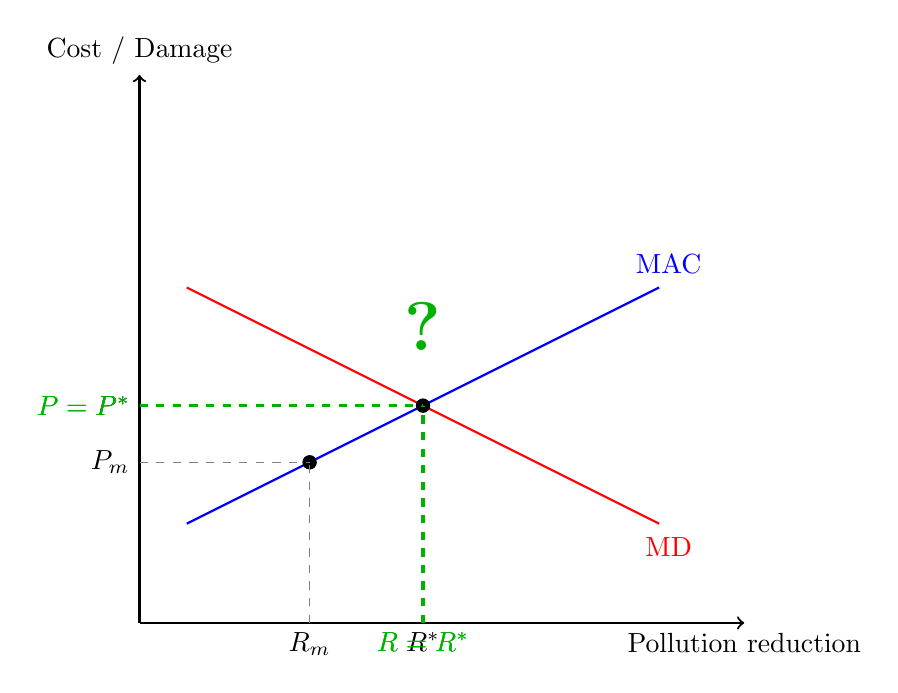
\begin{tikzpicture}[scale=1.2]
\pgfmathsetmacro{\m}{0.5}
\pgfmathsetmacro{\bA}{0.8}
\pgfmathsetmacro{\k}{3.8}
\pgfmathsetmacro{\Rstar}{(\k-\bA)/(2*\m)}
\pgfmathsetmacro{\Pstar}{\m*\Rstar+\bA}
\pgfmathsetmacro{\Rm}{\Rstar-1.2}
\pgfmathsetmacro{\Pm}{\m*\Rm+\bA}
% Axes
\draw[->, thick] (0,0) -- (6.4,0) node[below] {Pollution reduction};
\draw[->, thick] (0,0) -- (0,5.8) node[above] {Cost / Damage};
% MAC
\draw[thick, blue] (0.5, {\m*0.5+\bA}) -- (5.5, {\m*5.5+\bA});
\node[blue] at (5.6, {\m*5.5+\bA+0.25}) {MAC};
% MD
\draw[thick, red] (0.5, {\k-\m*0.5}) -- (5.5, {\k-\m*5.5});
\node[red] at (5.6, {\k-\m*5.5-0.25}) {MD};
% Optimum
\filldraw[black] (\Rstar,\Pstar) circle (2pt);
\draw[dashed, gray] (\Rstar,0) -- (\Rstar,\Pstar);
\draw[dashed, gray] (0,\Pstar) -- (\Rstar,\Pstar);
% Market level
\filldraw[black] (\Rm,\Pm) circle (2pt);
\draw[dashed, gray] (\Rm,0) -- (\Rm,\Pm);
\draw[dashed, gray] (0,\Pm) -- (\Rm,\Pm);
\node[below] at (\Rm,0) {$R_m$};
\node[left] at (0,\Pm) {$P_m$};

% 1) Quantity (vertical line in green)
\onslide<1>{
\draw[dashed, very thick, green!70!black] (\Rstar,0) -- (\Rstar,\Pstar);
\node[below, green!70!black] at (\Rstar,0) {$R = R^*$};
\node[left] at (0,\Pstar) {$P^*$};
}
% 2) Price (horizontal line in green)
\onslide<2>{
\draw[dashed, very thick, green!70!black] (0,\Pstar) -- (\Rstar,\Pstar);
\node[below] at (\Rstar,0) {$R^*$};
\node[left, green!70!black] at (0,\Pstar) {$P = P^*$};
}
% 3) Price + quantity + ?
\onslide<3>{
\draw[dashed, very thick, green!70!black] (\Rstar,0) -- (\Rstar,\Pstar);
\draw[dashed, very thick, green!70!black] (0,\Pstar) -- (\Rstar,\Pstar);
\node[below, green!70!black] at (\Rstar,0) {$R = R^*$};
\node[left, green!70!black] at (0,\Pstar) {$P = P^*$};
\node[green!70!black, font=\Huge\bfseries]
at (\Rstar,\Pstar) [yshift=1cm] {?};
}

\end{tikzpicture}
\end{frame}


%========================
% B: uncertainty
%========================
\begin{frame}[label=w7_uncertainty]{Uncertainty about abatement costs \& pollution damages}

\begin{itemize}
  \item<1-> With perfect information, $q^*$ and $p^*$ are known, and regulating the price or the quantity is equivalent.

  \item<2-> In reality, the social planner lacks information \& the costs and benefits of abatement are uncertain:
  \[
  MAC(q,\textcolor{blue}{\theta}) \quad ; \quad MD(q,\textcolor{red}{\eta}),
  \]
  where \textcolor{blue}{$\theta$} and \textcolor{red}{$\eta$} are uncertainty parameters.
\end{itemize}

\vspace{0.2cm}

\onslide<3->{
\textbf{Implication:}
\begin{itemize}
  \item<3-> The social planner's decisions are approximate, so necessarily imperfect (sub-optimal).
  \item<4-> E.g. $p_r<p^*$: too much pollution; $q_r > q^*$: too high costs.
  \item<5-> Trade-off: fixing $p_r$ gives ``cost certainty'', fixing $q_r$ gives ``damage certainty''.
\end{itemize}
}

\end{frame}


%========================
% B: comparison and approximation
%========================
\begin{frame}[label=w7_compare]{Comparing the price and the quantity instrument}
\onslide<1->{
\textbf{Comparison criterion $\Delta$ (``comparative advantage of prices'')}
\vspace{0.05cm}
\[
\Delta = W^{\text{price}} - W^{\text{quantity}}
\]
}
\onslide<2->{
\vspace{-0.2cm}
\[
\text{where } W^{\text{price}} = \mathbb{E}\Big[B\big(q(p,\textcolor{blue}{\theta}),\textcolor{red}{\eta}\big) - C\big(q(p,\textcolor{blue}{\theta}),\textcolor{blue}{\theta}\big)\Big].
\]
}
\only<3>{
\vspace{-0.6cm}
\begin{itemize}
  \item $\Delta > 0$: regulating the price is preferable.
  \item $\mathbb{E}$: expected welfare, the average over all possible realisations of costs and benefits.
\end{itemize}
\vspace{0.2cm}
}
\onslide<4->{
\textbf{Local approximation of $\Delta$}
\vspace{0.05cm}
\[
\Delta \approx \frac{\sigma^2}{2(C'')^2}\big(B'' + C''\big).
\]
\begin{itemize}
  \item $C''$: slope of the marginal abatement cost (MAC), positive,
  \item $B''$: slope of the marginal damage (MD), negative,
  \item $\sigma^2$: variance of the cost shock.
\end{itemize}
\vspace{0.05cm}
\textbf{Result:}
the sign of $B'' + C''$ determines the better instrument.
}
\end{frame}


\begin{frame}[label=w7_conclusion]{Conclusion: price vs quantity}

\textbf{Key result (Weitzman 1974)}
\begin{itemize}
    \item Regulate through \textbf{prices} or \textbf{quantities} depending on the slope of the MAC relative to the slope of the MD
\end{itemize}

\vspace{0.4cm}
\textbf{Limitations from the underlying assumptions}
\begin{enumerate}
    \item \textbf{Firm heterogeneity}: a quota without a permit market becomes more inefficient when MACs differ across firms.

    \item \textbf{Non-linear damages}: linearity is questionable given climate tipping points and potential irreversibility $\Rightarrow$ favours regulating quantities.
\end{enumerate}

\vspace{0.4cm}
\textbf{Conclusion:} no definitive verdict on which instrument is superior, but a useful framework to understand the trade-offs.

\end{frame}

% =====================================================================
% PART C: MAC and MD against EMISSIONS (not abatement), 25 Nov 2026
% Replaces the cropped handout picture on the lecture slide "Marginal
% abatement cost vs marginal damage". Mirror image of frame w7_mac_md:
% the x-axis is emissions, so MAC falls and MD rises.
%   MAC = 0.8 (5 - e): zero at e^m = 5 (no abatement without regulation)
%   MD  = 0.2 + 0.6 e
%   e^* = (4 - 0.2)/1.4 = 2.71 ; P^* = 0.2 + 0.6*2.71 = 1.83
%   a = remaining damage (under MD, 0 to e^*)
%   b = total abatement cost (under MAC, e^* to e^m)
% Export (handout PDF, last page):
%   py "$HOME/.claude/skills/latex-teaching/scripts/export_frames.py" lecture07_weitzman_handout.pdf
%      --out ../png/week7 --pages 12 --names w7_mac_md_emissions
% =====================================================================
\begin{frame}[label=w7_mac_md_emissions]{Marginal abatement cost vs marginal damage}
\centering
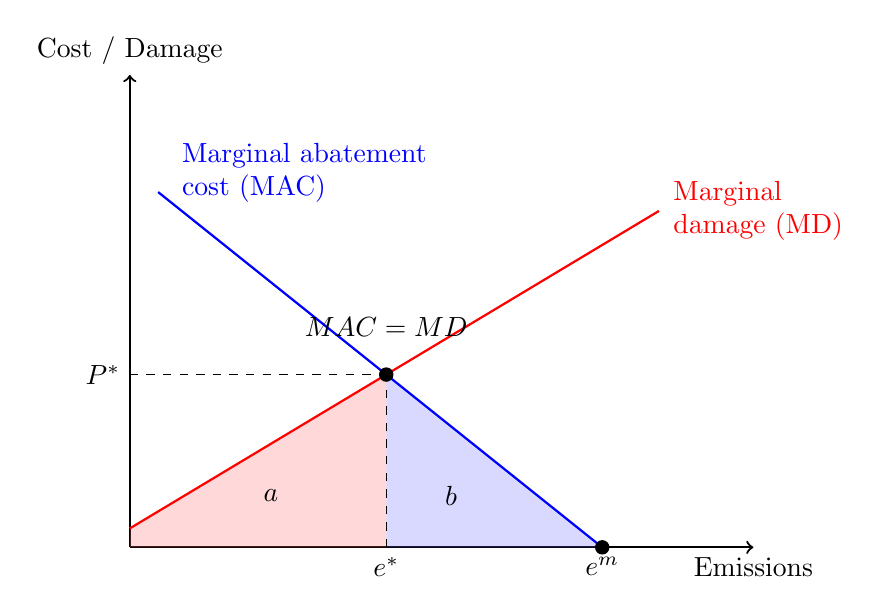
\begin{tikzpicture}[scale=1.2]

% Parameters
\pgfmathsetmacro{\mA}{0.8}   % slope of MAC (falls with emissions)
\pgfmathsetmacro{\eM}{5.0}   % emissions without regulation: MAC = 0
\pgfmathsetmacro{\bD}{0.2}   % intercept MD
\pgfmathsetmacro{\mD}{0.6}   % slope of MD

% Optimum: MAC = MD
\pgfmathsetmacro{\eStar}{(\mA*\eM-\bD)/(\mA+\mD)}
\pgfmathsetmacro{\Pstar}{\bD+\mD*\eStar}

% Axes (always visible)
\draw[->, thick] (0,0) -- (6.6,0) node[below] {Emissions};
\draw[->, thick] (0,0) -- (0,5.0) node[above] {Cost / Damage};

% 4) Areas: a = remaining damage, b = total abatement cost (drawn first, under the curves)
\onslide<5->{
\fill[red!60, opacity=0.25] (0,0) -- (0,\bD) -- (\eStar,\Pstar) -- (\eStar,0) -- cycle;
\fill[blue!60, opacity=0.25] (\eStar,0) -- (\eStar,\Pstar) -- (\eM,0) -- cycle;
\node at ({\eStar*0.55}, {\Pstar*0.3}) {$a$};
\node at ({\eStar+(\eM-\eStar)*0.3}, {\Pstar*0.3}) {$b$};
}

% 1) MAC
\onslide<2->{
\draw[thick, blue] (0.3, {\mA*(\eM-0.3)}) -- (\eM, 0);
\node[blue, right, align=left] at (0.45, {\mA*(\eM-0.3)+0.2}) {Marginal abatement \\ cost (MAC)};
\filldraw[black] (\eM,0) circle (2pt);
\node[below] at (\eM,0) {$e^m$};
}
% 2) MD
\onslide<3->{
\draw[thick, red] (0, \bD) -- (5.6, {\bD+\mD*5.6});
\node[red, right, align=left] at (5.65, {\bD+\mD*5.6}) {Marginal \\ damage (MD)};
}
% 3) Optimum
\onslide<4->{
\filldraw[black] (\eStar,\Pstar) circle (2pt);
\draw[dashed] (\eStar,0) -- (\eStar,\Pstar);
\node[below] at (\eStar,0) {$e^*$};
\draw[dashed] (0,\Pstar) -- (\eStar,\Pstar);
\node[left] at (0,\Pstar) {$P^*$};
}
\onslide<4>{
\node[above] at (\eStar, \Pstar + 0.3) {$MAC = MD$};
}

\end{tikzpicture}
\end{frame}

\end{document}
